\documentclass[conference]{IEEEtran}
\usepackage{amsmath,amssymb,amsfonts,amsthm}
\usepackage{graphicx}
\usepackage{textcomp}
\usepackage{xcolor}
\usepackage{hyperref}
\usepackage{booktabs}
\usepackage{subcaption}

\begin{document}

\title{SafeContract: A Practitioner's Toolkit for\\VLA Action-Space Monitoring}

\author{\IEEEauthorblockN{Krishnam Gupta}
\IEEEauthorblockA{Independent Research \\
San Francisco, CA \\
kayjee1994@gmail.com}}

\maketitle

\begin{abstract}
Vision-Language-Action models ship with zero action-space safety infrastructure.
OpenVLA sends raw outputs to motors with no bounds checking; pi0 streams via WebSocket with no validation; LeRobot's safety processor is imperative and easy to omit.
We present \texttt{SafeContract}, a training-free, black-box toolkit that adds calibrated action monitoring to any VLA in four lines of Python.
Across three architectures (VQ-BeT, Diffusion Policy, ACT) and two environments (PushT 2D, ALOHA 14-DOF bimanual), we find that \emph{different architectures need different monitors}: direction reversal rate is a universal failure predictor (AUROC 0.93, 0.79, 0.91), jerk predicts failure only for discrete-token models (0.88 vs.\ 0.43), and velocity violations alone are non-predictive (0.41--0.69).
Split-conformal calibration from demonstrations eliminates hand-tuned thresholds (97.9\% coverage), and CUSUM shift detection catches degradation within 7 steps.
SafeContract enforces and monitors at 13\,$\mu$s per step - less than 0.001\% of typical VLA inference time - with no model access, no retraining, and no task degradation ($p \ge 0.68$ across all experiments).\footnote{Code and results: \url{https://github.com/krishnam94/vla-edge}}
\end{abstract}

\begin{IEEEkeywords}
VLA deployment, action-space monitoring, safety toolkit, conformal prediction, failure prediction
\end{IEEEkeywords}

\section{Introduction: The Deployment Gap}

VLA models~\cite{openvla,smolvla} predict robot actions end-to-end from vision and language.
The field has invested heavily in making these models more capable, but virtually nothing in making their outputs safe at deployment time.
Consider the current state of practice:

\begin{itemize}
    \item OpenVLA's deployment script sends raw action outputs directly to motors with zero bounds checking~\cite{openvla}.
    \item pi0 streams actions via WebSocket with no validation layer~\cite{pi0}.
    \item LeRobot's~\cite{lerobot} \texttt{EEBoundsAndSafety} processor is imperative, non-composable, and trivially omitted.
    \item SmolVLA produces actions up to 3.7$\times$ outside $[-1, 1]$ bounds on LIBERO~\cite{libero}.
\end{itemize}

\noindent The implicit assumption is: if the model is good enough, the actions will be safe enough.
We show this assumption is wrong, and that it is wrong in \emph{architecture-specific} ways that a one-size-fits-all monitor cannot catch.

\textbf{This paper answers one question: ``I am deploying a VLA tomorrow. What should I do?''}
We provide (1) a four-step deployment workflow, (2) architecture-matched monitor recommendations backed by controlled experiments, and (3) an open-source toolkit that implements the full pipeline in four lines of Python.

Our contributions:
\begin{enumerate}
    \item \textbf{Architecture-matched monitoring recommendations.} Same-dataset experiments ($n{=}200$ episodes, same seeds) show VQ-BeT produces 2.4$\times$ more velocity violations than Diffusion Policy, and the best monitor differs by architecture family (Table~\ref{tab:crossarch}).
    \item \textbf{A universal failure predictor.} Direction reversal rate achieves AUROC ${=}$ 0.93 (VQ-BeT), 0.79 (Diffusion), and 0.91 (ACT/ALOHA 14-DOF) - the only monitor predictive across all three architectures.
    \item \textbf{Data-driven calibration that replaces hand-tuning.} Split-conformal bounds~\cite{vovk2005} achieve 97.9\% coverage; CUSUM~\cite{page1954} detects degradation within 7 steps. No hand-tuned thresholds, no model internals.
\end{enumerate}

\section{Deployment Workflow}
\label{sec:workflow}

SafeContract turns VLA deployment monitoring into four steps (Fig.~\ref{fig:workflow}).

\noindent\textbf{Step 1: Calibrate from demonstrations.}
\texttt{SafetyGuard.from\_demos(demo\_actions)} computes split-conformal bounds ($\alpha{=}0.05$) and per-joint velocity limits (99th percentile of consecutive deltas) from your demonstration data.
No manual threshold tuning.
At $\alpha{=}0.05$, conformal bounds are 25\% tighter than the 4$\sigma$ heuristic while providing 97.9\% holdout coverage (99.1\% minimum per dimension).

\noindent\textbf{Step 2: Select monitors for your architecture.}
Consult Table~\ref{tab:recipe}.
If your VLA uses discrete tokens (VQ-BeT, OpenVLA), enable jerk and reversal monitors.
If it uses continuous denoising (Diffusion, flow matching), enable stall detection and reversal monitors.
If you are unsure, enable all monitors - the overhead is negligible.

\noindent\textbf{Step 3: Wrap your predict function.}

{\small
\begin{verbatim}
guard = SafetyGuard.from_demos(demo_actions)

@guard.wrap  # bounds + velocity + stall + jerk
def predict(obs):
    return model(obs)

# Every call is now monitored and enforced.
action = predict(obs)
status = guard.status()  # p-value, CUSUM, flags
\end{verbatim}
}

\noindent The decorator clips to calibrated bounds, clamps velocity, and logs all violations with timestep, dimension, and magnitude.
Overhead: 13\,$\mu$s per call ($<$0.001\% of VLA inference).

\noindent\textbf{Step 4: Monitor CUSUM during rollout.}
The conformal p-value stream feeds a CUSUM detector that accumulates evidence of distribution shift.
When CUSUM exceeds threshold $h$, the system signals degradation.
Response options: reduce $v_{\max}$, switch to a fallback controller, or request human intervention.
On ALOHA demonstrations, in-distribution actions produce zero alarms; adding $\sigma{=}0.1$ noise triggers detection within 7 steps ($h{=}3$).

\begin{figure}[t]
    \centering
    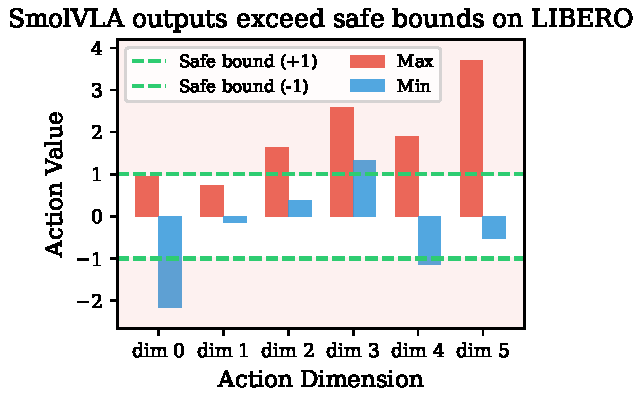
\includegraphics[width=\columnwidth]{figures/fig1_action_ranges.pdf}
    \caption{SmolVLA action ranges on 100 LIBERO observations. Most dimensions exceed $[-1, 1]$ bounds (green dashes), confirming that VLAs produce unsafe actions that monitoring would catch.}
    \label{fig:workflow}
\end{figure}

\section{Method}
\label{sec:method}

\subsection{Safety Contracts and Enforcement}

A safety contract $C = (\mathbf{l}, \mathbf{u}, v_{\max})$ specifies per-joint bounds and a velocity limit:
$l_i \leq a_i \leq u_i$ for each joint $i$, and $\|\mathbf{a}_t - \mathbf{a}_{t-1}\|_\infty \leq v_{\max}$.
Enforcement proceeds in three phases: (1)~clip to per-joint bounds, (2)~clamp velocity, (3)~re-clip to bounds.
The final re-clip is critical: velocity clamping can push actions outside original bounds.
For hyperrectangular contracts $C_1, C_2$, sequential clipping equals intersection clipping, so stacking decorators is order-independent.

\subsection{Conformal Calibration}
\label{sec:calibration}

Hand-tuned thresholds are unreliable: $v_{\max}{=}0.05$ clips a significant fraction of \emph{expert} actions on ALOHA.
Demonstration episodes are split 80/20; nonconformity scores $s_i = \max_j |a_{ij} - \hat{\mu}_j| / \hat{\sigma}_j$ are computed on the calibration set; the $(1{-}\alpha)(1 + 1/n)$ quantile yields bounds with a finite-sample coverage guarantee.
Velocity limits are set per-joint at the 99th percentile of consecutive action deltas.

Each action also receives a conformal p-value: $p(s) = |\{i : s_i \ge s\}| / (n+1)$.
Under exchangeability, $P(p \le \alpha) \le \alpha$ - a proper statistical test, not a heuristic~\cite{vovk2005}.
The p-value stream feeds CUSUM~\cite{page1954}: $S_t = \max(0, S_{t-1} + \mathbf{1}[p_t < \alpha] - \alpha)$, which is Lorden-optimal for detecting persistent mean shifts, with a formal false-alarm bound that EWMA cannot provide.

\subsection{Architecture-Specific Monitors}
\label{sec:monitors}

Bounds and velocity alone miss architecture-specific failure modes.
SafeContract includes four targeted monitors:

\noindent\textbf{Direction reversal rate.}
For each joint $j$, a reversal occurs when $\text{sign}(\Delta a_{t,j}) \neq \text{sign}(\Delta a_{t-1,j})$.
The episode rate averages over all (timestep, joint) pairs.
High reversal rates indicate indecisive, oscillatory behavior.
This is the single most predictive monitor across all architectures we tested.

\noindent\textbf{Jerk monitoring.}
The third derivative of the action trajectory detects denoising artifacts in diffusion policies and chunk boundary discontinuities in action-chunked models~\cite{acg2025}.
Strongly predictive for discrete-token architectures; less so for continuous denoisers.

\noindent\textbf{Stall detection.}
Flags when $\|\mathbf{a}_t - \mathbf{a}_{t-1}\|_2 < \tau$ for $w$ consecutive steps.
Catches policy freeze - the primary failure mode of diffusion policies~\cite{safe2025} - which is invisible to bounds/velocity monitoring.

\noindent\textbf{Gripper oscillation.}
Rapid open/close cycling ($>k$ flips in $w$ steps) signals grasp indecision in bimanual manipulation.
Individual transitions pass velocity checks, but the pattern is pathological.

\section{Experiments}
\label{sec:experiments}

Platform: RunPod GPU cluster, Python 3.12.
Full monitoring overhead: $<$0.001\% of typical VLA inference time (${\sim}$13\,$\mu$s per call).

\subsection{VLAs Produce Unsafe Actions}
\label{sec:exp_unsafe}

SmolVLA on 100 LIBERO observations: after correct MEAN\_STD unnormalization, bounds violations drop from 86\% to 0\% - every bounds violation was a normalization bug, detectable by monitoring.
The robust finding is velocity: at $v_{\max}{=}0.1$ rad/step, \textbf{98\%} of SmolVLA steps violate versus \textbf{16\%} of expert steps - a 6$\times$ gap that persists regardless of normalization.
Bounds monitoring catches integration bugs; velocity monitoring catches physical safety concerns.

\subsection{Cross-Architecture Comparison}
\label{sec:crossarch}

We evaluate three architectures on their respective tasks, using conformal calibration from demonstrations (Step 1) and the same per-architecture evaluation protocol.

\textbf{Diffusion Policy}~\cite{diffusionpolicy} (262M, PushT, $n{=}200$, seeds 0--199).
Without SafeContract: 58\% success.
With: 57\% ($p = 0.92$).
772 violations caught, zero task degradation.

\textbf{VQ-BeT}~\cite{vqbet} (37.5M, PushT, $n{=}200$, same seeds).
Without: 56.5\%.
With: 54.5\% ($p = 0.76$).
1,847 violations - 2.4$\times$ more than Diffusion on the same task.

\textbf{ACT}~\cite{act} (51.6M, ALOHA 14-DOF bimanual, $n{=}50$).
Without: 62\%.
With: 56\% ($p = 0.68$).
4,758 violations caught.

Across all three, SafeContract enforces without statistically significant task degradation.

\subsection{Which Monitors Work for Which Architecture?}
\label{sec:monitors_results}

Table~\ref{tab:crossarch} presents failure prediction AUROCs.
The key findings for practitioners:

\textbf{Always enable reversal rate monitoring.}
It predicts failure with AUROC 0.93 (VQ-BeT), 0.79 (Diffusion), and 0.91 (ACT/ALOHA).
It is the only monitor that is strongly predictive ($p < 0.001$) across all three architectures and both action dimensionalities (2D and 14-DOF).

\textbf{Enable jerk monitoring for discrete-token VLAs.}
Jerk AUROC follows a discrete-to-continuous gradient: 0.88 (VQ-BeT), 0.69 (ACT), 0.43 (Diffusion).
For autoregressive token-based VLAs (OpenVLA, VQ-BeT), jerk captures quantization artifacts at token boundaries.
For smooth denoisers, jerk is non-predictive.

\textbf{Do not rely on velocity violations alone.}
Velocity AUROC ranges from 0.41 to 0.69 - not useful as a standalone failure predictor for any architecture.

\begin{figure}[t]
    \centering
    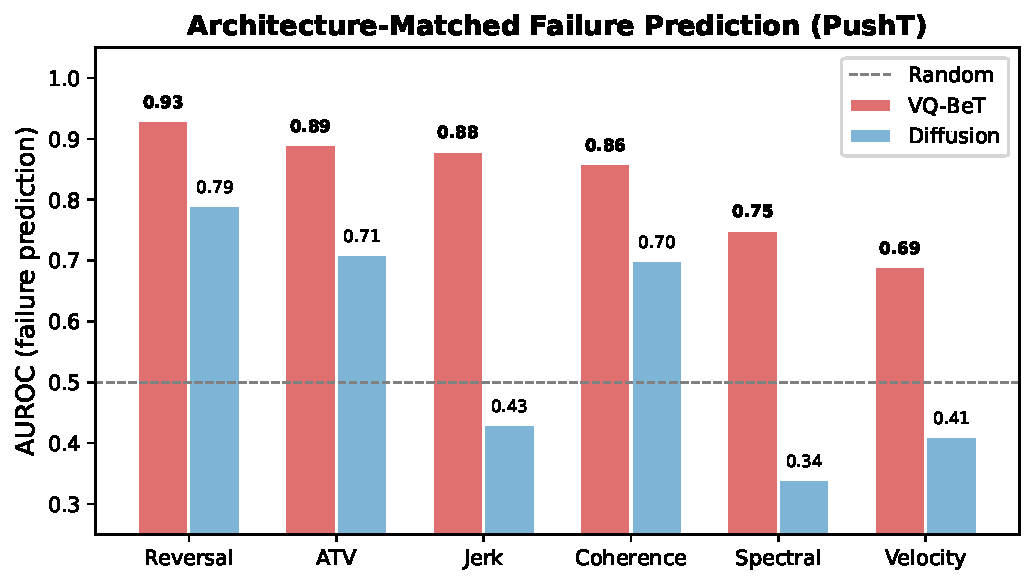
\includegraphics[width=\columnwidth]{figures/fig_auroc_comparison.pdf}
    \caption{Monitor effectiveness varies by architecture. Reversal rate is the universal predictor. Jerk works for discrete-token models (VQ-BeT) but not continuous denoisers (Diffusion). No single monitor is best everywhere.}
    \label{fig:auroc}
\end{figure}

\begin{figure}[t]
    \centering
    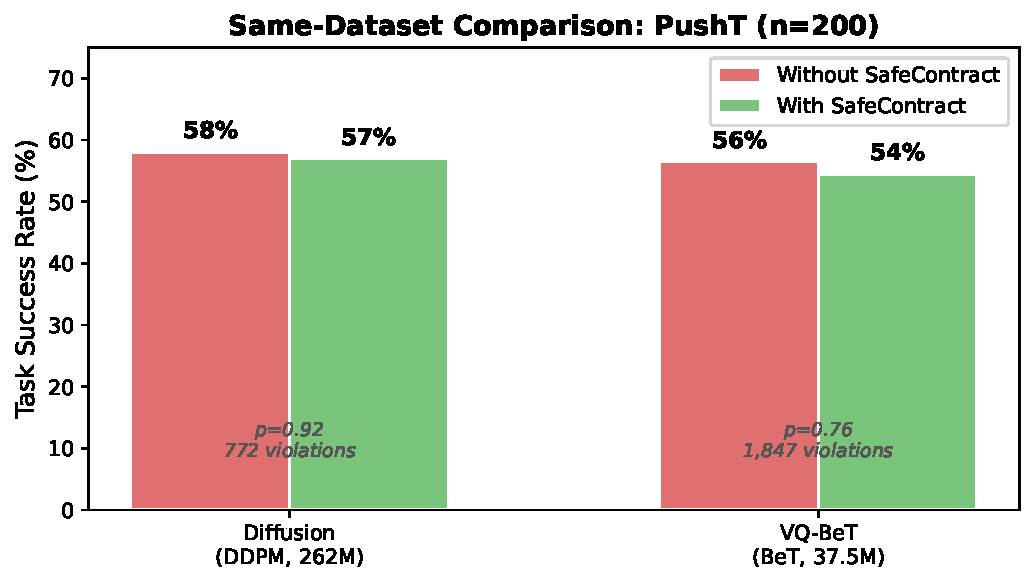
\includegraphics[width=\columnwidth]{figures/fig_pusht_comparison.pdf}
    \caption{Same-dataset comparison on PushT ($n{=}200$). SafeContract catches 772 (Diffusion) and 1,847 (VQ-BeT) violations with no task degradation ($p{=}0.92$, $p{=}0.76$).}
    \label{fig:closedloop}
\end{figure}

\begin{table*}[t]
\centering
\caption{Cross-architecture results with failure prediction AUROCs and practitioner recommendations. PushT: $n{=}200$ per condition (same seeds/contract), AUROCs on $n{=}100$. ALOHA: $n{=}50$ per condition, AUROCs on $n{=}50$.}
\label{tab:crossarch}
\small
\begin{tabular}{lccc}
\toprule
 & \textbf{Diffusion (PushT)} & \textbf{VQ-BeT (PushT)} & \textbf{ACT (ALOHA 14-DOF)} \\
\midrule
Family & Continuous (DDPM) & Discrete (VQ-VAE + Transformer) & Continuous (chunked) \\
Params & 262M & 37.5M & 51.6M \\
Success (no / with contract) & 58\% / 57\% & 56.5\% / 54.5\% & 62\% / 56\% \\
Fisher's $p$ & 0.92 & 0.76 & 0.68 \\
Violations caught & 772 & \textbf{1{,}847} & 4{,}758 \\
\midrule
AUROC: reversal rate & 0.79 & \textbf{0.93} & \textbf{0.91} \\
AUROC: jerk & 0.43 & \textbf{0.88} & 0.69 \\
AUROC: momentum coherence & 0.70 & \textbf{0.86} & 0.71 \\
AUROC: spectral energy & 0.34 & \textbf{0.75} & 0.74 \\
AUROC: velocity & 0.41 & 0.69 & 0.52 \\
\midrule
\textbf{Recommended monitors} & reversal, stall, coherence & reversal, jerk, spectral & reversal, jerk, gripper osc. \\
\textbf{Primary failure mode} & policy freeze (stall) & token boundary jitter & chunk boundary + grasp indecision \\
\textbf{Watch for} & micro-movements, no progress & high-frequency oscillation & gripper cycling, arm drift \\
\bottomrule
\end{tabular}
\end{table*}

\section{Practical Recommendations}
\label{sec:recommendations}

Table~\ref{tab:recipe} summarizes monitor selection by VLA architecture family.
The recommendations extend beyond the three architectures we tested: they are grounded in the structural properties (discrete vs.\ continuous action generation, chunked vs.\ per-step) that determine failure modes.

\begin{table}[t]
\centering
\caption{Monitor recipes by VLA family. Start with your architecture row. Enable the listed monitors. Watch for the listed failure mode.}
\label{tab:recipe}
\small
\begin{tabular}{p{1.4cm}p{2.9cm}p{2.9cm}}
\toprule
\textbf{VLA Family} & \textbf{Enable These Monitors} & \textbf{Failure Mode to Watch} \\
\midrule
Discrete token\newline\scriptsize{(VQ-BeT, OpenVLA)} & reversal rate, jerk, spectral energy & High-freq oscillation at token boundaries \\
\midrule
Diffusion / flow\newline\scriptsize{(Diffusion, pi0)} & reversal rate, stall, momentum coherence & Policy freeze: valid-looking micro-movements \\
\midrule
Action-chunked\newline\scriptsize{(ACT, GR00T)} & reversal rate, jerk, gripper oscillation & Chunk boundary discontinuity, grasp cycling \\
\midrule
Hybrid AR+diff\newline\scriptsize{(pi0.5, CogACT)} & all monitors & Semantically correct trajectory toward wrong target \\
\bottomrule
\end{tabular}
\end{table}

\textbf{Deployment integration.}
SafeContract operates at the action output layer, between the VLA's \texttt{predict()} and the robot's motor commands.
It is agnostic to the middleware above (ROS 2, LeRobot, OpenPI, direct motor control) and below (Jetson, GPU server, cloud).
For ROS 2, wrap the action callback.
For LeRobot, decorate the policy's \texttt{select\_action()}.
For direct motor control, insert between inference and the motor driver.

\textbf{Where SafeContract fits in a full monitoring stack.}
A production VLA deployment needs monitoring at multiple levels~\cite{kim2026guardrails}: workspace constraints (CBFs), task progress (semantic monitors), perception consistency, and more.
SafeContract is \emph{Layer 0} - the innermost, fastest check on raw action outputs.
It composes with CBF-based workspace constraints~\cite{aegis}, task-level monitors~\cite{sentinel}, and perception-level failure detectors~\cite{fiper2025} as part of defense-in-depth.
Its value is that it requires nothing except action outputs: no dynamics model, no model internals, no auxiliary training.

\section{Related Work}

\textbf{Training-time safety.}
SafeVLA~\cite{safevla} and RobustVLA~\cite{robustvla} improve safety via retraining or fine-tuning.
Complementary to runtime monitoring - a policy can be both trained safely and monitored at deployment.

\textbf{Inference-time safety.}
AEGIS~\cite{aegis} solves a CBF-QP per step (requires dynamics models); SafeDiffuser~\cite{safediffuser} and CoDiG~\cite{codig} embed barriers in diffusion (architecture-specific); SafeDec~\cite{safedec} constrains decoding; Safety Chip~\cite{safetychip} uses LTL monitors; ATACOM~\cite{atacom} projects onto constraint manifolds.
All require either dynamics models, architecture access, or retraining.
SafeContract requires none of these.

\textbf{Failure detection.}
SAFE~\cite{safe2025} and FIPER~\cite{fiper2025} train auxiliary models on VLA features for failure detection; Sentinel~\cite{sentinel} monitors temporal consistency.
These detect failures but do not prevent them.
SafeContract both detects (via monitors) and prevents (via enforcement).

\textbf{Conformal prediction for robotics.}
Recent work validates conformal prediction for robot safety~\cite{safe2025,feldman2025}.
Kim et al.~\cite{kim2026guardrails} argue that modular guardrails are necessary for foundation-model robots.
SafeContract provides a concrete, calibrated, open-source implementation.

\section{Discussion}
\label{sec:discussion}

\textbf{The central result is a practical recipe, not just an empirical finding.}
VLA architectures fail in architecture-specific ways (Table~\ref{tab:crossarch}), and the monitors that predict failure are architecture-specific (Table~\ref{tab:recipe}).
A practitioner deploying a discrete-token VLA should watch jerk; a practitioner deploying a diffusion VLA should watch for stalls.
Both should always monitor reversal rate.

\textbf{Regulatory motivation.}
The EU AI Act (Article 9) mandates continuous monitoring for high-risk AI systems by 2027.
Robots operating near humans qualify.
SafeContract provides auditable telemetry - per-step violation logs, conformal p-values, CUSUM alarm history - that supports compliance without requiring model transparency.

\textbf{What SafeContract cannot catch.}
Hybrid architectures (autoregressive reasoning plus diffusion actions) can produce physically valid trajectories toward the wrong target.
No action-space monitor can detect this.
Semantic correctness requires perception-level~\cite{fiper2025} and task-level~\cite{sentinel} monitoring above SafeContract in the stack.

\textbf{Limitations.}
(1)~All experiments are in simulation; real-robot patterns may differ.
(2)~Three of eleven known VLA architecture families tested; autoregressive (OpenVLA) and flow matching (pi0) are untested but predicted by the discrete/continuous gradient.
(3)~Conformal coverage (97.9\%) holds under exchangeability with calibration data; during rollout, coverage degrades under distribution shift. CUSUM detects when this occurs; adaptive conformal inference~\cite{gibbs2021} would maintain coverage online.

\textbf{Future work.}
Extending to autoregressive and flow-matching architectures,
real-robot validation on physical hardware,
adaptive conformal inference~\cite{gibbs2021} for online recalibration,
and integration with ROS 2 safety lifecycle management.

\begin{thebibliography}{20}
\bibitem{openvla} Kim, M.J. et al., ``OpenVLA: An Open-Source Vision-Language-Action Model,'' CoRL 2024, arXiv:2406.09246.
\bibitem{smolvla} Shukor, M. et al., ``SmolVLA: A Vision-Language-Action Model for Affordable and Efficient Robotics,'' arXiv:2506.01844, 2025.
\bibitem{lerobot} Cadene, R. et al., ``LeRobot: State-of-the-art Machine Learning for Real-World Robotics in PyTorch,'' 2024, \url{https://github.com/huggingface/lerobot}.
\bibitem{pi0} Black, K. et al., ``$\pi_0$: A Vision-Language-Action Flow Model for General Robot Control,'' arXiv:2410.24164, 2024.
\bibitem{libero} Liu, B. et al., ``LIBERO: Benchmarking Knowledge Transfer for Lifelong Robot Learning,'' NeurIPS 2023.
\bibitem{safevla} Zhang, B. et al., ``SafeVLA: Towards Safety Alignment of Vision-Language-Action Model via Constrained Learning,'' NeurIPS 2025, arXiv:2503.03480.
\bibitem{aegis} Hu, S. et al., ``VLSA: Vision-Language-Action Models with Plug-and-Play Safety Constraint Layer,'' arXiv:2512.11891, 2025.
\bibitem{safedec} Kapoor, P. et al., ``Constrained Decoding for Robotics Foundation Models,'' arXiv:2509.01728, 2025.
\bibitem{robustvla} Guo, J. et al., ``On Robustness of VLA Models against Multi-Modal Perturbations,'' ICLR 2026.
\bibitem{safetychip} Yang, Z. et al., ``Plug in the Safety Chip: Enforcing Constraints for LLM-driven Robot Agents,'' ICRA 2024.
\bibitem{safediffuser} Xiao, W. et al., ``SafeDiffuser: Safe Planning with Diffusion Probabilistic Models,'' ICLR 2025.
\bibitem{codig} Ma, H. et al., ``CoDiG: Constraint-Aware Diffusion Guidance for Robotics,'' CoRL 2025.
\bibitem{atacom} Tolle, M. et al., ``Towards Safe Robot Foundation Models Using Inductive Biases,'' arXiv:2505.10219, 2025.
\bibitem{sentinel} Agia, C. et al., ``Unpacking Failure Modes of Generative Policies: Runtime Monitoring of Consistency and Progress,'' CoRL 2024, arXiv:2410.04640.
\bibitem{vovk2005} Vovk, V. et al., ``Algorithmic Learning in a Random World,'' Springer, 2005.
\bibitem{page1954} Page, E.S., ``Continuous Inspection Schemes,'' Biometrika 41(1/2):100--115, 1954.
\bibitem{safe2025} Gu, Q. et al., ``SAFE: Multitask Failure Detection for Vision-Language-Action Models,'' NeurIPS 2025, arXiv:2506.09937.
\bibitem{fiper2025} Romer, R. et al., ``Failure Prediction at Runtime for Generative Robot Policies,'' NeurIPS 2025, arXiv:2510.09459.
\bibitem{feldman2025} Feldman, A.O. et al., ``Conformal Safety Monitoring for Flight Testing,'' arXiv:2511.20811, 2025.
\bibitem{gibbs2021} Gibbs, I. and Candes, E., ``Adaptive Conformal Inference Under Distribution Shift,'' NeurIPS 2021, arXiv:2106.00170.
\bibitem{acg2025} Park, M. et al., ``ACG: Action Coherence Guidance for Flow-based VLA Models,'' arXiv:2510.22201, 2025.
\bibitem{kim2026guardrails} Kim, J. et al., ``Modular Safety Guardrails Are Necessary for Foundation-Model-Enabled Robots in the Real World,'' arXiv:2602.04056, 2026.
\bibitem{diffusionpolicy} Chi, C. et al., ``Diffusion Policy: Visuomotor Policy Learning via Action Diffusion,'' RSS 2023, arXiv:2303.04137.
\bibitem{vqbet} Lee, S. et al., ``Behavior Generation with Latent Actions,'' ICML 2024, arXiv:2403.03181.
\bibitem{act} Zhao, T.Z. et al., ``Learning Fine-Grained Bimanual Manipulation with Low-Cost Hardware,'' RSS 2023, arXiv:2304.13705.
\end{thebibliography}

\end{document}
